\subsection{Business Case}
\subsubsection{Den nuværende situation}
\subparagraph{Timeregistrering til regning}

    Hver fredag udfylder svendene en papirsskabelon, hvor de skriver stedet arbejdet er blevet udført, hvilken dag arbejdet er udført, hvad der er gjort, hvilke materialer der er taget fra firmaets eget værksted, og hvor mange timer der er brugt.
    Dette gøres for alle timerne i ugen.
    
    Hver tirsdag eller onsdag samler sekretæren alle deres registreringer og skriver regninger til Halvorsen's kunder.

\subparagraph{Timeregistrering til aflønning}
    Hver anden fredag udfylder svendene også en anden papirsskabelon, hvor de skriver alle 14 dage, og hvor mange timer de har arbejdet de enkelte dage. Overarbejdstimer skrives separat.
    
    For både regning og aflønningstimeregistreringen er svendene derfor nød til at køre tilbage på værkstedet for at udfylde papirerne.

Et BPMN diagram over denne proces kan ses på figur \ref{fig:BPMN}.
    
\begin{figure}
    \makebox[\textwidth][c]{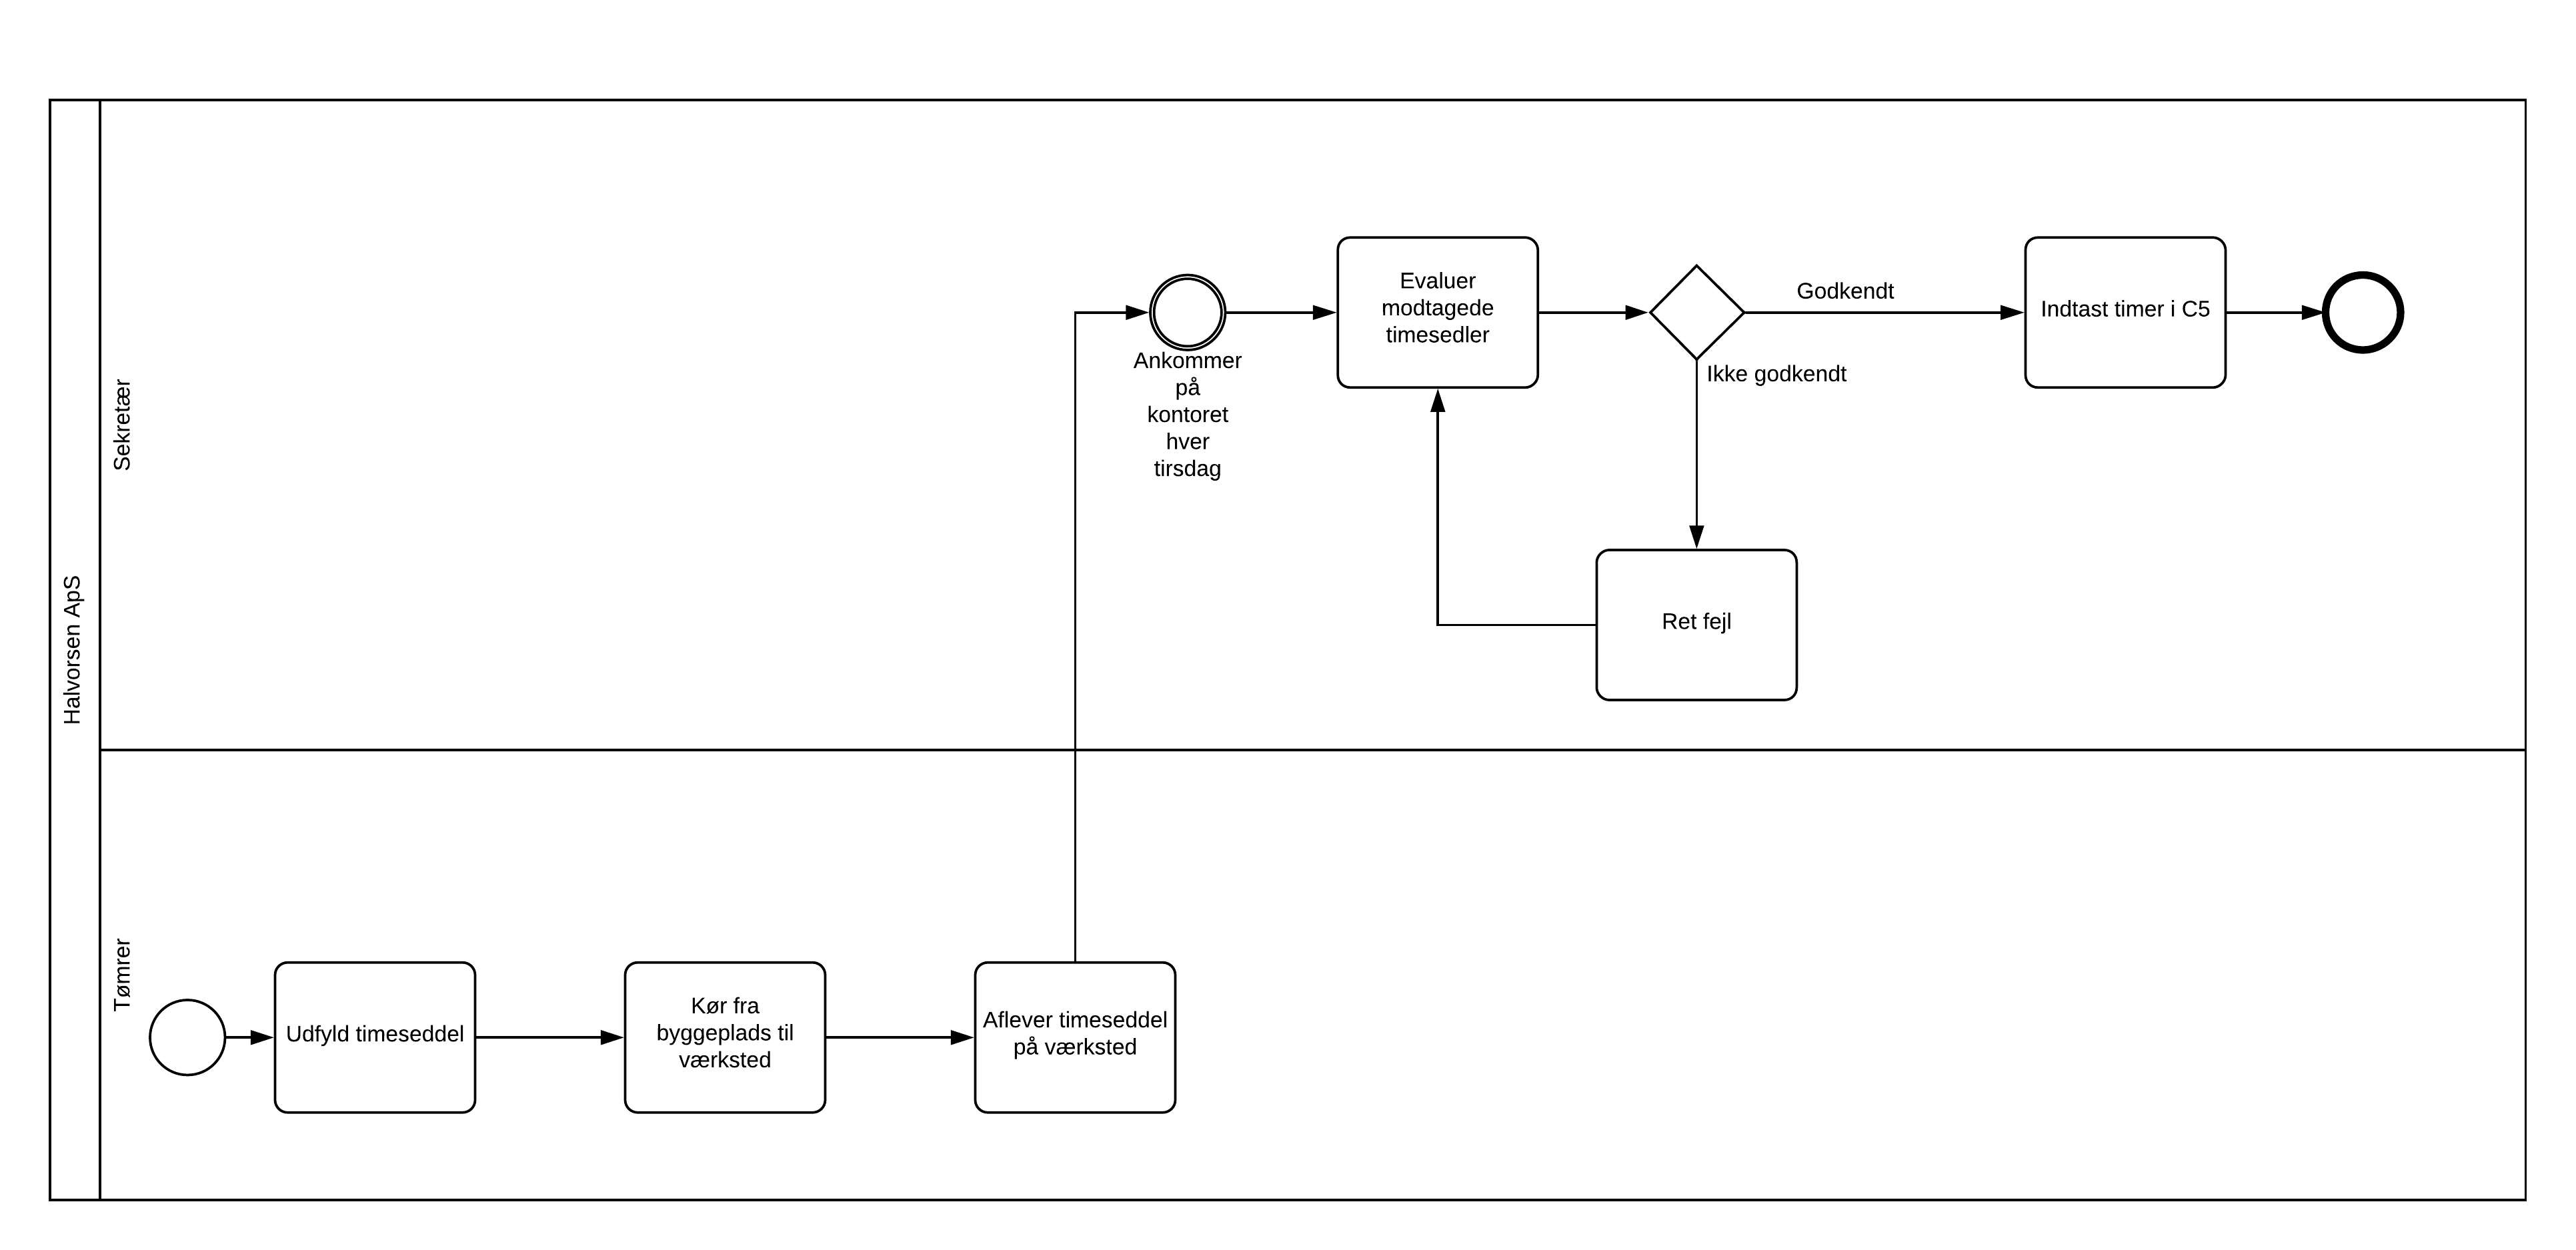
\includegraphics[scale = 0.6]{BPMN.png}}
    \caption{BPMN for tidsregistrering}
    \label{fig:BPMN}
\end{figure}
    
\subparagraph{Intern materialebestilling}
    Når en svend opdager, at der mangler materiale på en byggeplads, som de skal bruge, ringer de hjem til tømmermesteren, hvor de fortæller, hvad de skal bruge, samt hvor og hvornår det skal bruges.
    
    Derfor skal Torben selv huske på alle bestillingerne.
    
\subparagraph{Arbejdstegninger}
    Svendene har arbejdstegninger i papirform med i deres biler ud på byggepladserne.
    Det betyder, at over tid bliver tegningerne krøllede og beskidte.
    Der er heller ikke mulighed for at forstørre en lille del op, så man nemmere kan se præcis, hvad der står på tegningen.
    
\subsubsection{Formålet med projektet}
    Projektet skal effektivisere den interne kommunikation i     firmaet.
    Dette gøres ved at arbejde med to problematikker.
    
    Først skal projektet sørge for, at tidsregistreringen kan foregå andre steder end hjemme på værksedet og derved spare spildt kørselstid.
    
    Dernæst skal projektet gøre det nemmere at bestille materialer fra deres eget værksted.
\subsubsection{Løsningsscenarier}

\begin{table}[H]
\centering
\begin{tabular}{@{}cl@{}}
\toprule
\textbf{Fordele}                                                                                                                         & \multicolumn{1}{c}{\textbf{Ulemper}}                                                                                                                          \\ \midrule
\multicolumn{2}{|c|}{\textbf{Fortsæt som normalt}}                                                                                                                                                                                                                                                       \\ \midrule
\multicolumn{1}{|l|}{\begin{tabular}[c]{@{}l@{}}Ingen ekstra udgifter.\\ Ingen omstillingsperiode.\end{tabular}}                         & \multicolumn{1}{l|}{Ingen optimering ved hjælp af IT.}                                                                                                        \\ \midrule
\multicolumn{2}{|c|}{\textbf{Køb af allerede eksisterende løsning f.eks Navision}}                                                                                                                                                                                                                       \\ \midrule
\multicolumn{1}{|l|}{\begin{tabular}[c]{@{}l@{}}Løsningen eksistere allerede.\\ Mulighed for køb af support.\end{tabular}}               & \multicolumn{1}{l|}{\begin{tabular}[c]{@{}l@{}}Stejl indlæringskurve\\ Dyr løsning\\ Alle problemer løses ikke\end{tabular}}                                  \\ \midrule
\multicolumn{2}{|c|}{\textbf{Email skabelon}}                                                                                                                                                                                                                                                            \\ \midrule
\multicolumn{1}{|l|}{Simpelt at sætte op}                                                                                                & \multicolumn{1}{l|}{\begin{tabular}[c]{@{}l@{}}Alle problemer løses ikke.\\ Stor risiko for menneskelige fejl.\end{tabular}}                                  \\ \midrule
\multicolumn{2}{|c|}{\textbf{\begin{tabular}[c]{@{}c@{}}App til Smartphone og Tablet\\ (Den valgte løsning)\end{tabular}}}                                                                                                                                                                               \\ \midrule
\multicolumn{1}{|l|}{\begin{tabular}[c]{@{}l@{}}Løsningen kan skræddersyes og udvides\\ til at opfylde virksomhedens krav.\end{tabular}} & \multicolumn{1}{l|}{\begin{tabular}[c]{@{}l@{}}De er nød til at anskaffe endtenarbejdstelefoner\\ til medarbejderne eller tablets til hver bil.\end{tabular}} \\ \bottomrule
\end{tabular}
\end{table}

\subsubsection{Interessentanalyse}
Mette og tømrermesteren Torben er som sekretær og tømrermester samt virksomhedsledere involveret i udviklingen af produktet, især Mette da hun skal bruge programmet for bogholderi, og Torben skal bruge det til det daglige arbejde.

Svendene skal også involveres i projektet til tider, eftersom programmet skal bruges af dem og løsningen omhandler dem.

For både Torben og hans svende gælder det, at de alle er en del af det grå guld, og de derfor ikke er vokset op med IT systemer som en fast del af deres liv.
Derfor er det vigtigt, at løsningen er intuitiv og nem at bruge for dem, ellers er det ikke muligt for systemet at optimere deres hverdag.
